\section{Numerical Results}
\label{sec:numerical_results}

\begin{frame}[c]{Synthetic Asset}
	\begin{block}{Goal}
		Evaluate different RL algorithms in a controlled environment, i.e.  on a synthetic asset with profitably tradable features 
	\end{block}
	The synthetic asset price is given by
	\begin{equation*}
		Z_t = \exp\left(\frac{z_t}{\max_t z_t - \min_t z_t}\right)
	\end{equation*}
	where $\{z_t\}$ is a random walk with autoregressive trend $\{\beta_t\}$
		\begin{equation*}
			\begin{split}
				z_t &= z_{t-1} + \beta_{t-1} + \kappa \epsilon_t\\
				\beta_t &= \alpha \beta_{t-1} + \nu_t\\
			\end{split}
		\end{equation*}
\end{frame}

\begin{frame}[c]{Convergence of RL algorithms}
\begin{figure}[t!]
	\centering
	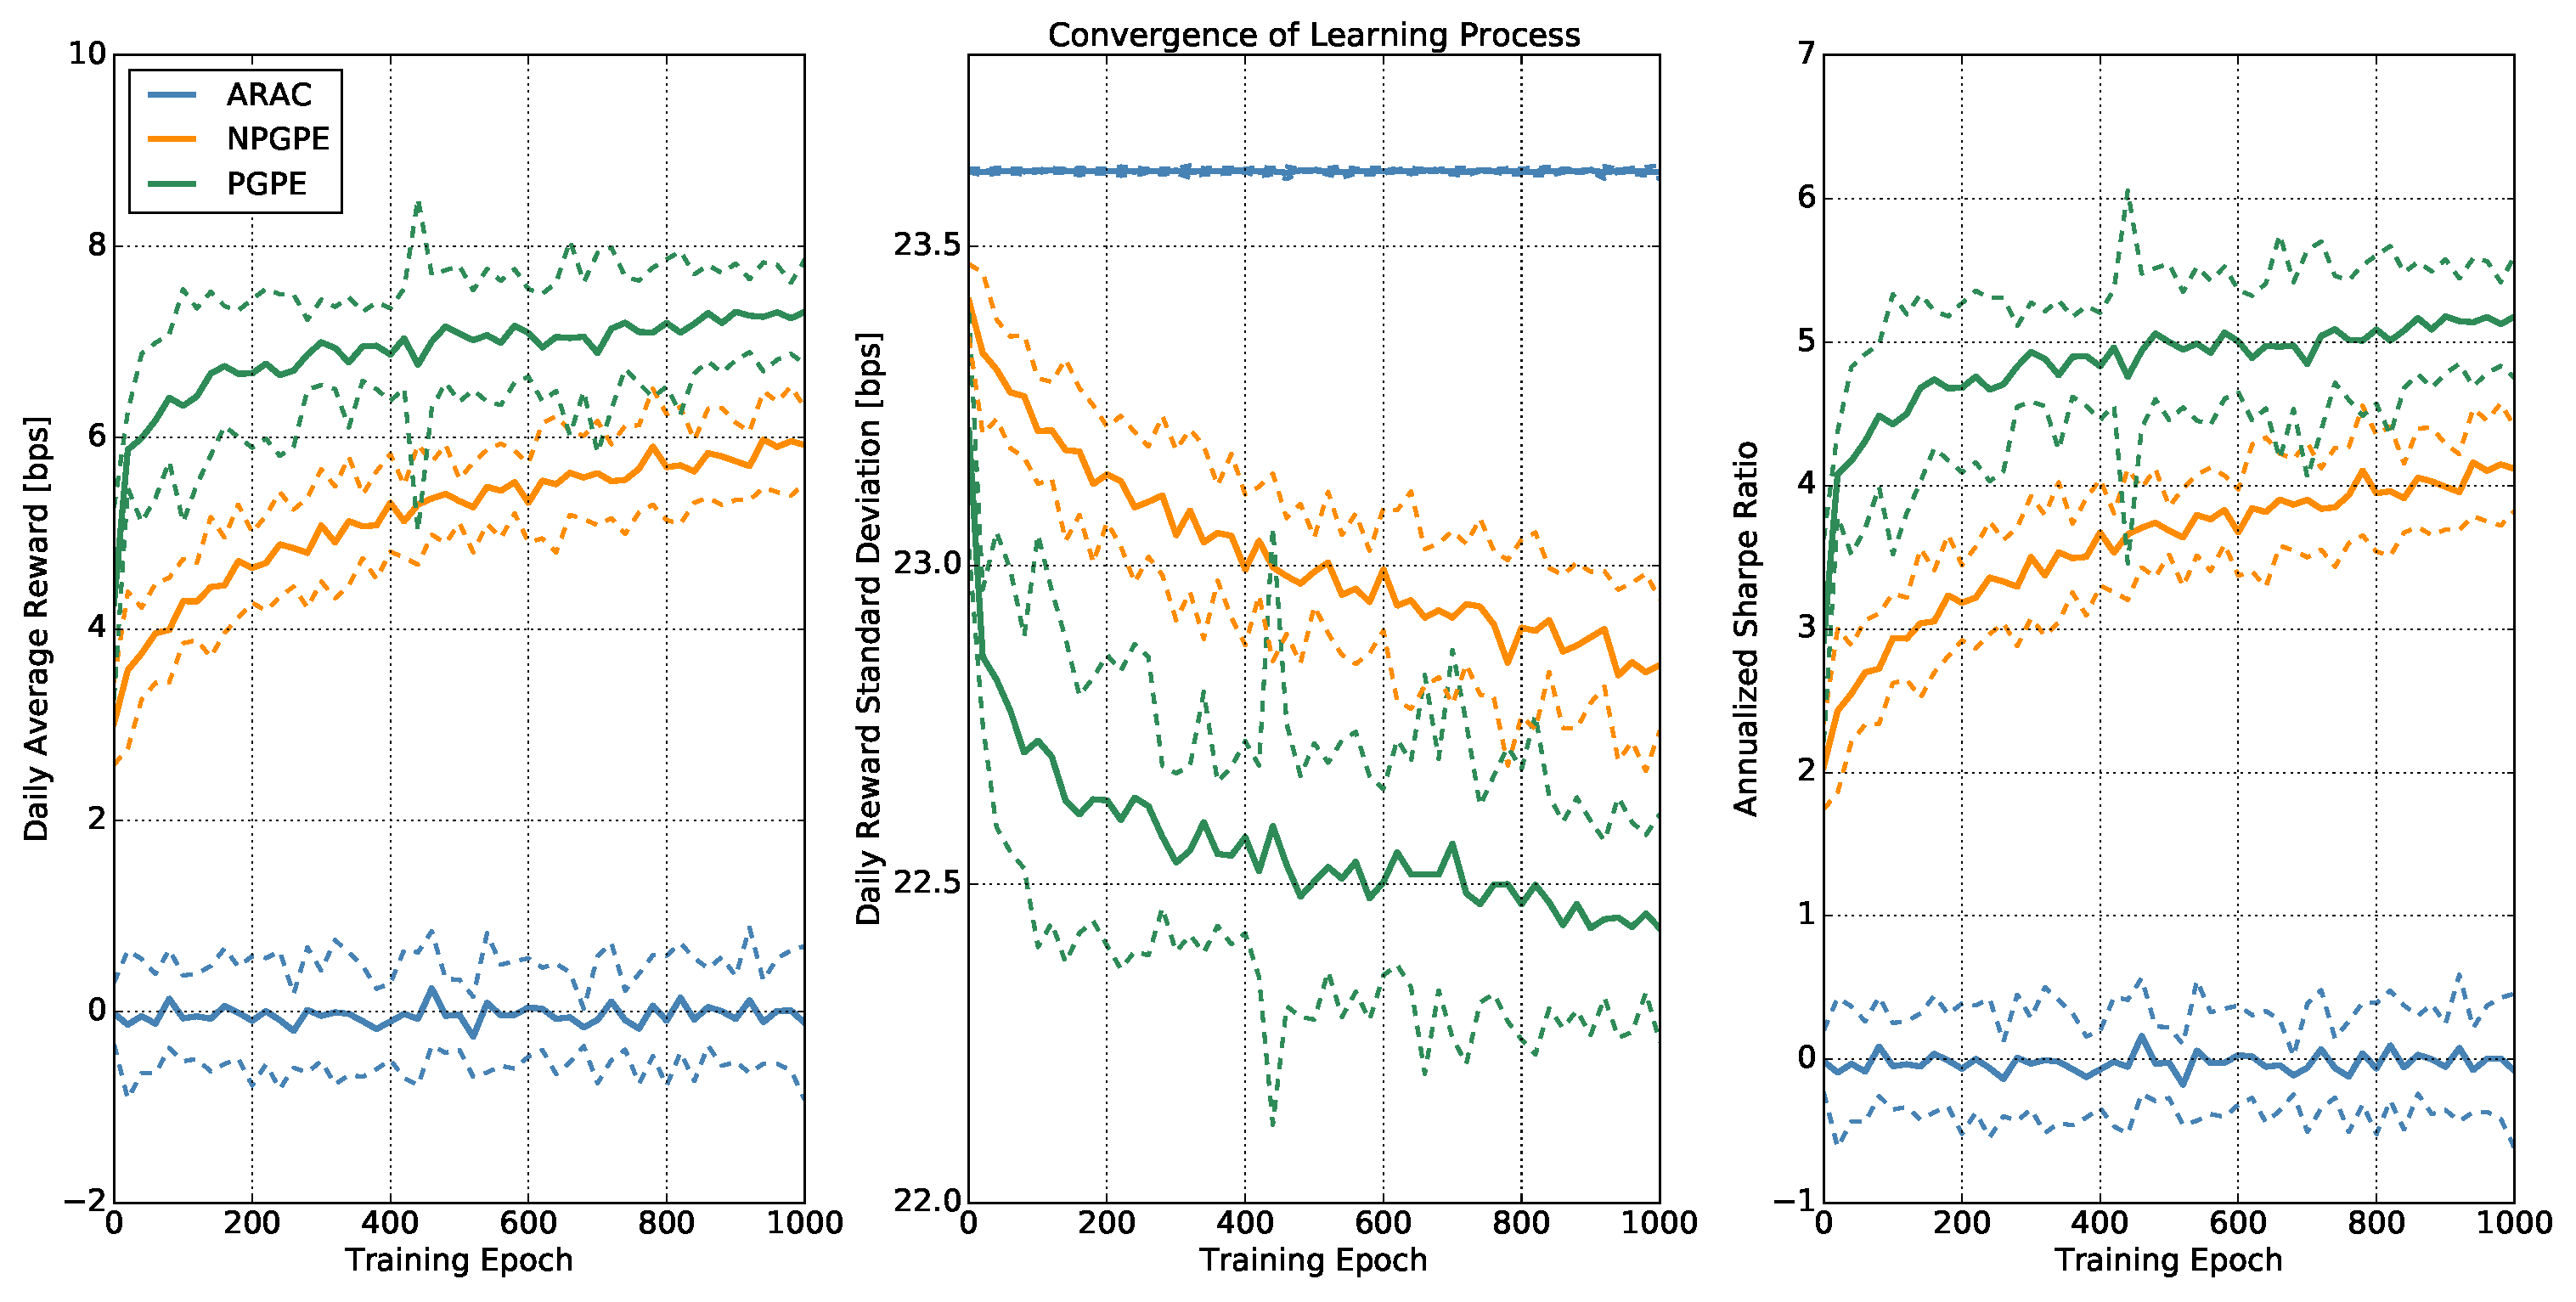
\includegraphics[height=5cm,width=1.0\textwidth]{Images/6_0_single_synthetic_neutral_convergence}
\end{figure}
\end{frame}


\begin{frame}[c]{Backtest Performance of the Trading Strategies Learned}
\begin{figure}[t]
	\centering
	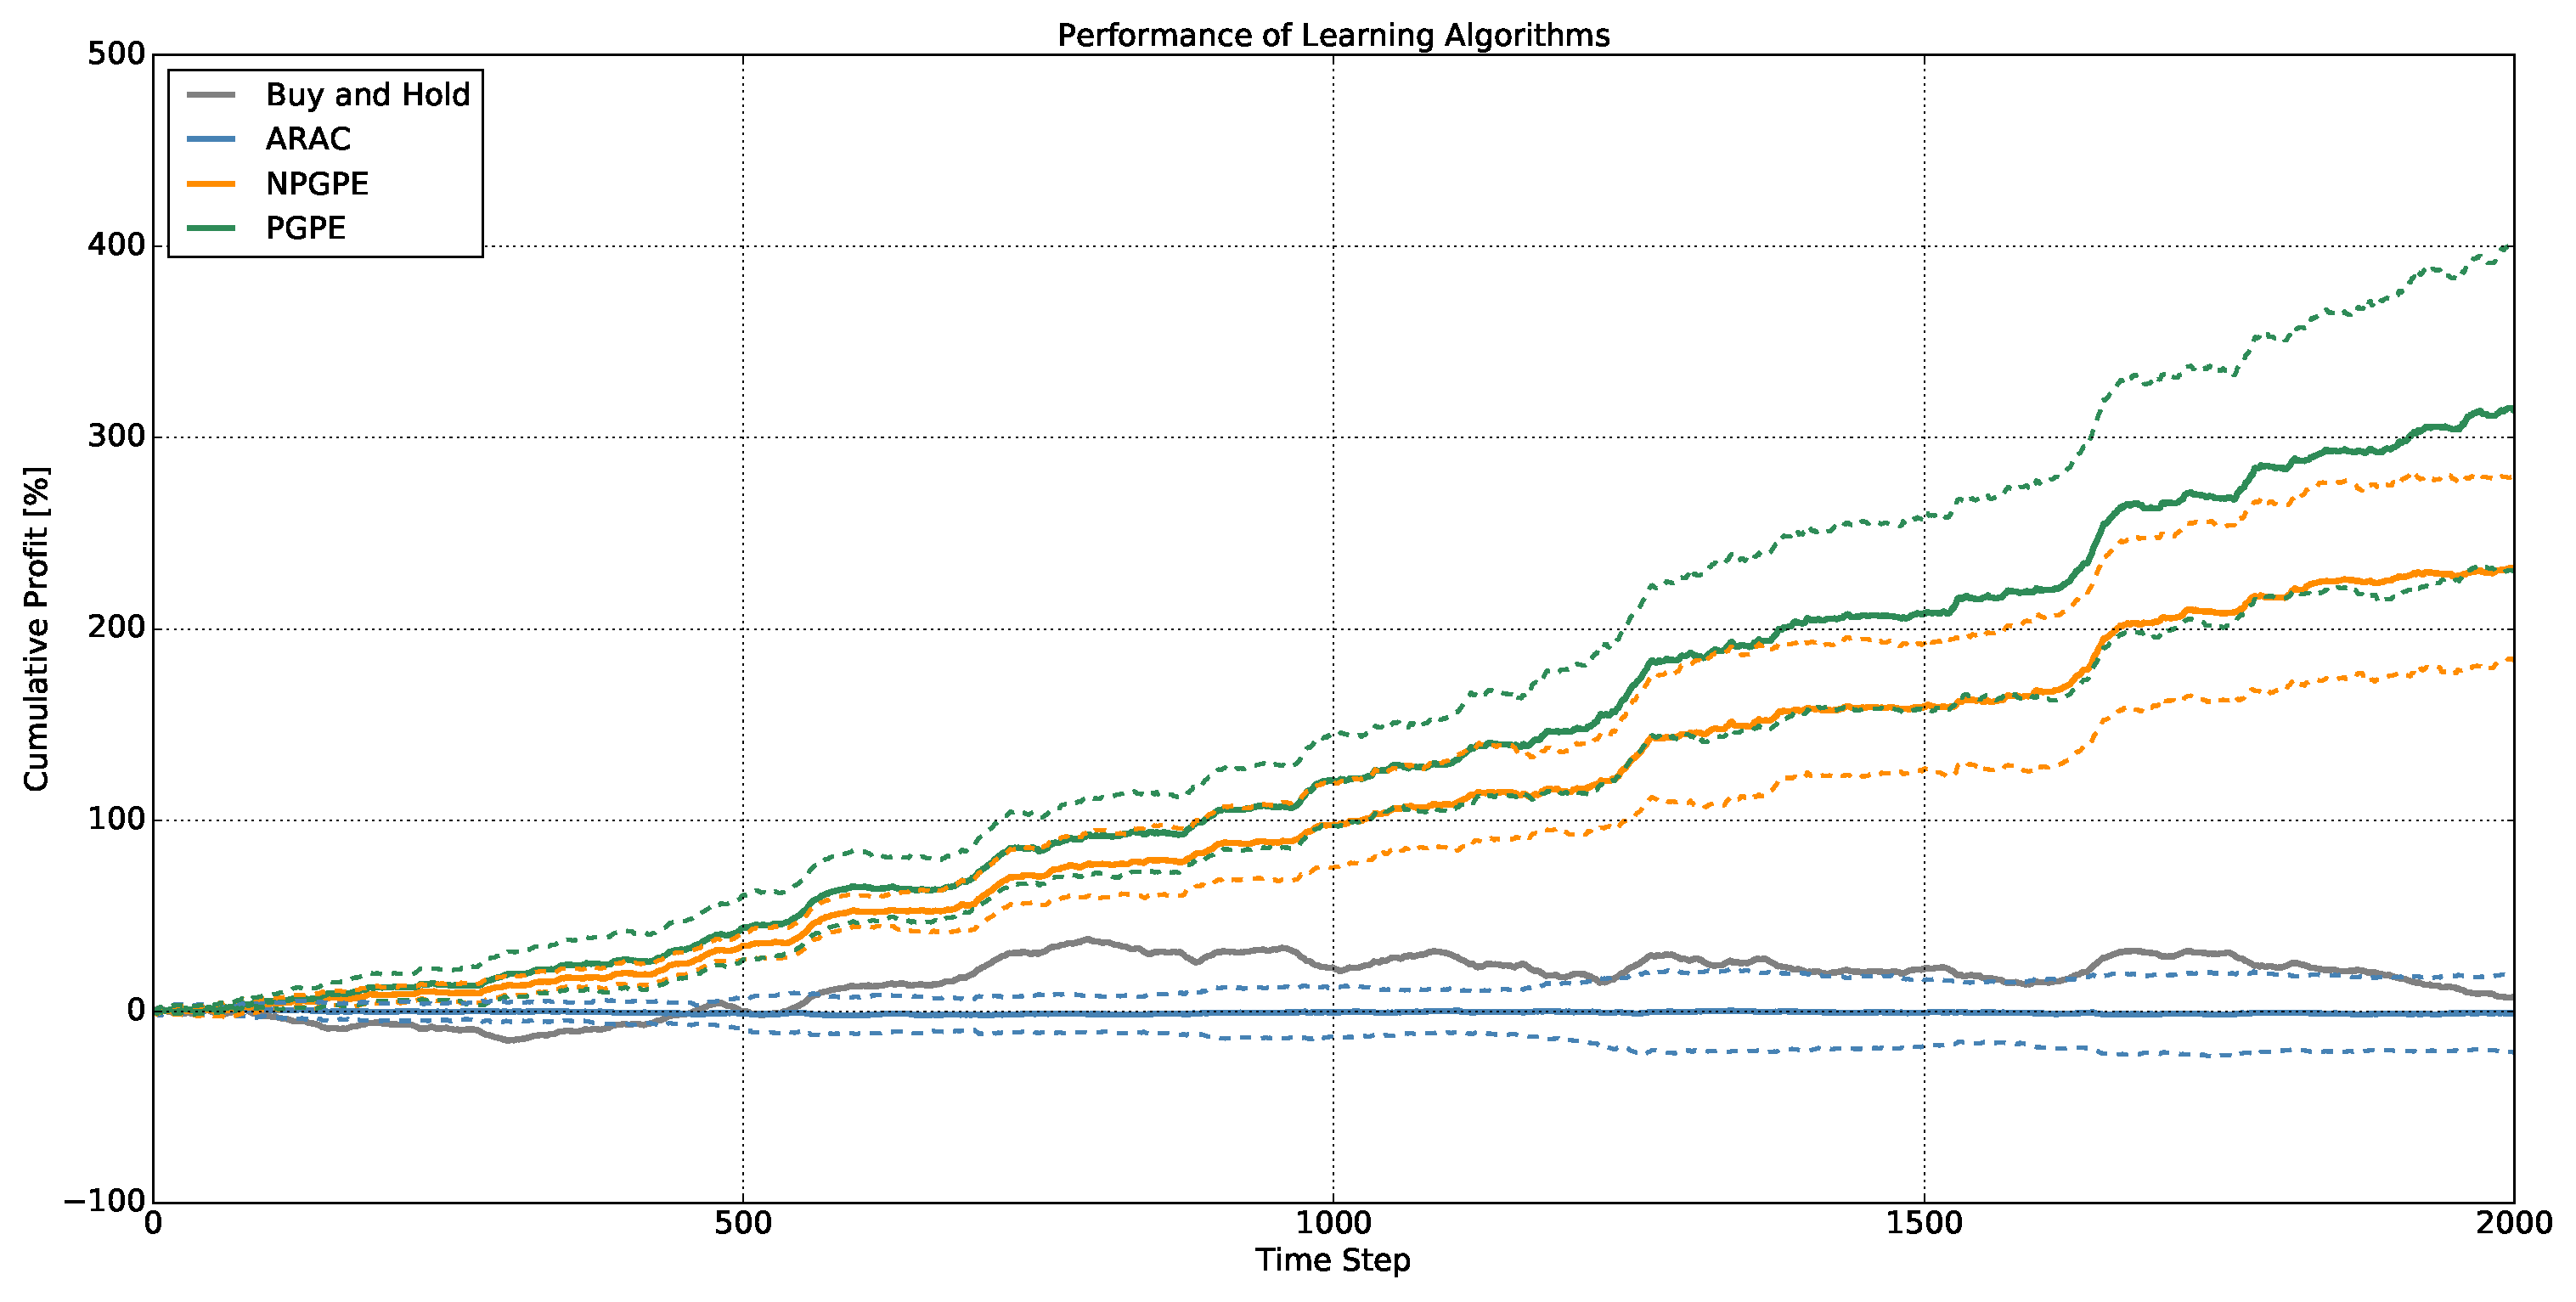
\includegraphics[height=6cm,width=1.0\textwidth]{Images/6_1_single_synthetic_neutral_performance}
\end{figure}
\end{frame}

\begin{frame}[c]{Impact of Transaction Costs}
\begin{figure}[t!]
	\centering
	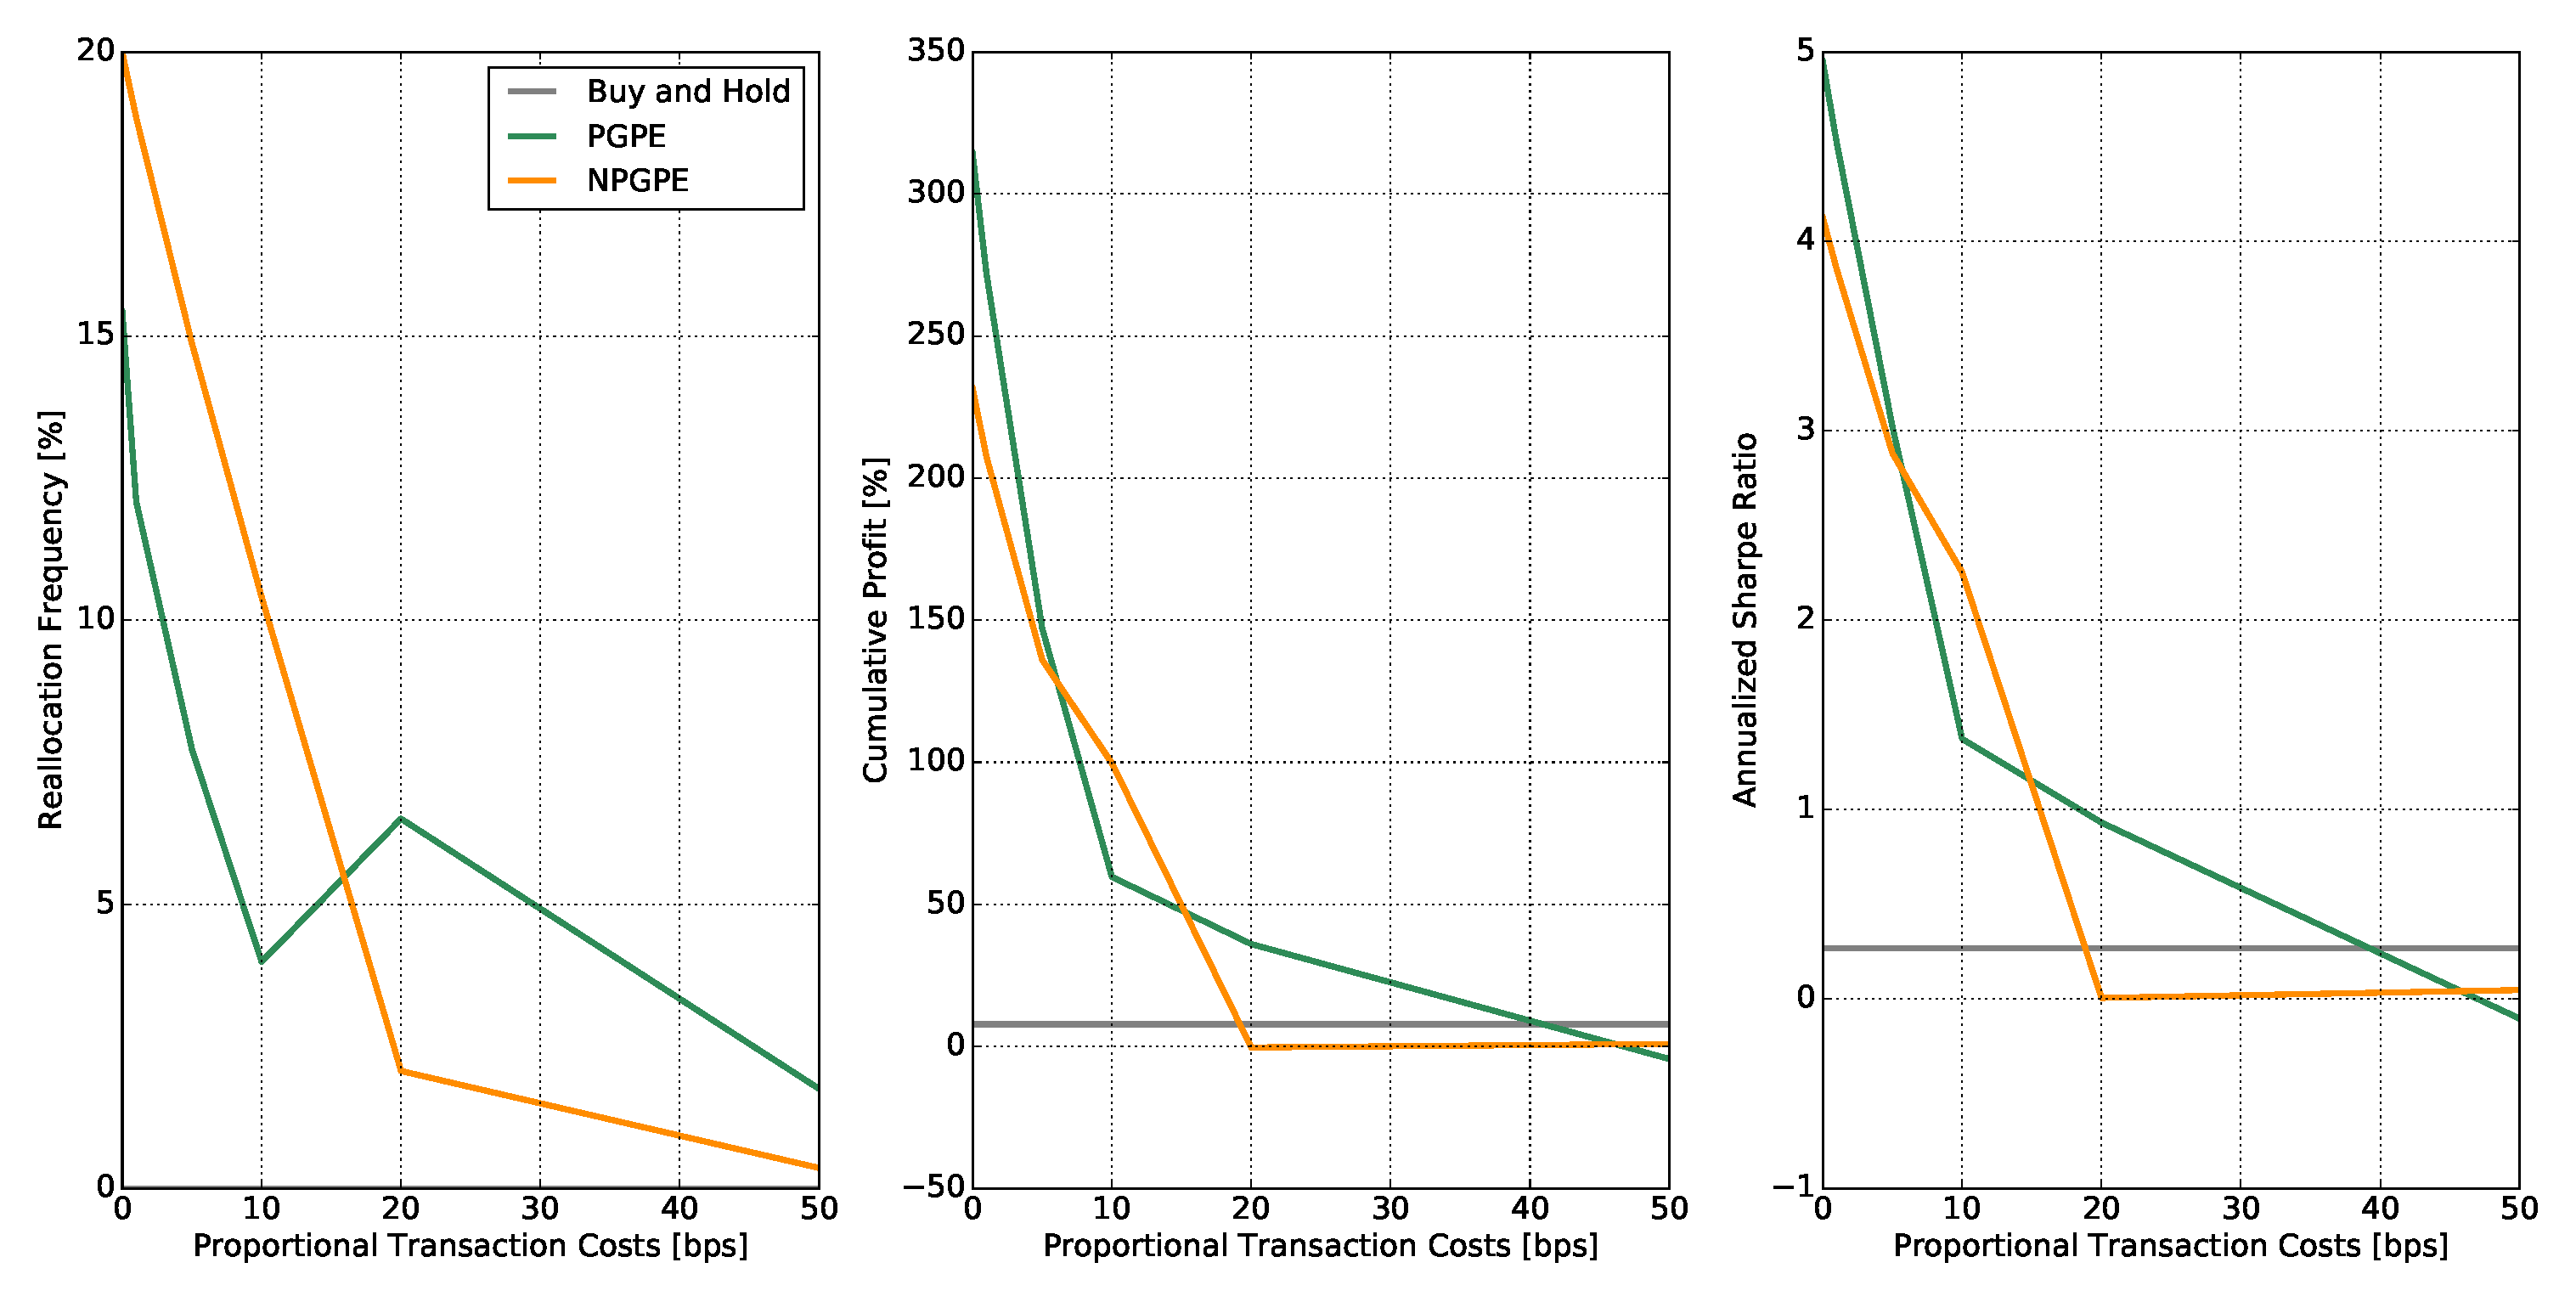
\includegraphics[height=3cm,width=1.0\textwidth]{Images/6_2_impact_transaction_costs}
\end{figure}
\begin{figure}[t!]
	\centering
	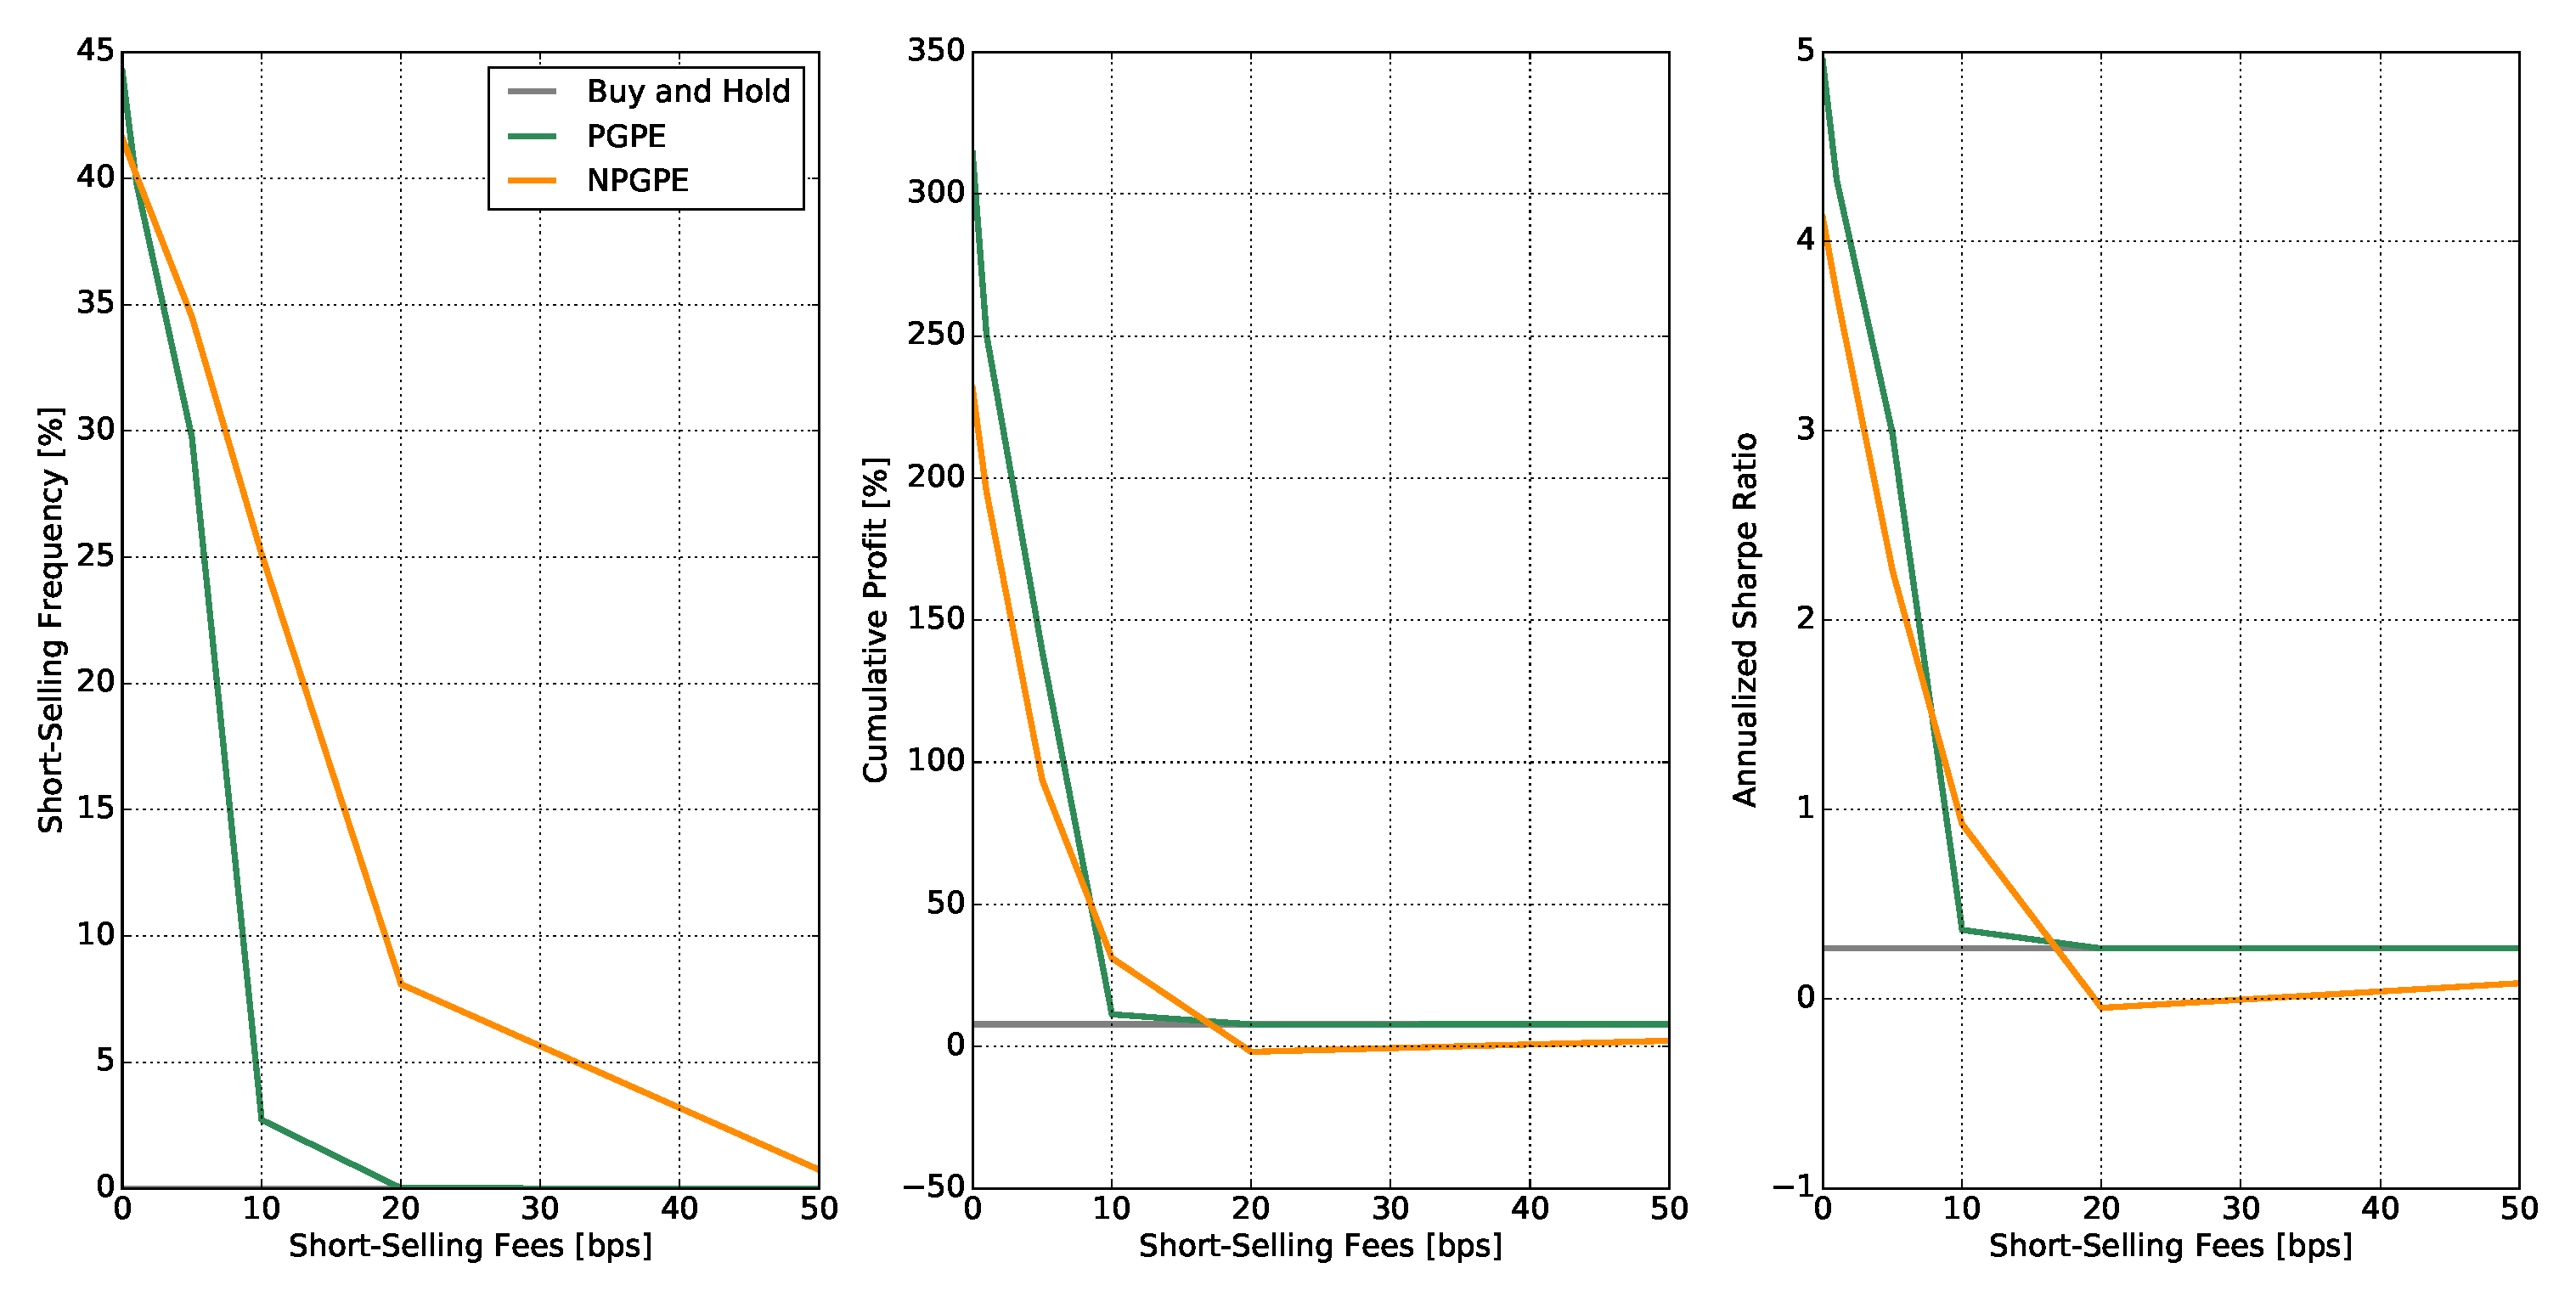
\includegraphics[height=3cm,width=1.0\textwidth]{Images/6_3_impact_short_selling_fees}
\end{figure}
\end{frame}


